% Author: Izaak Neutelings (November 2020)
\documentclass[border=3pt,tikz]{standalone}
\usepackage{physics}
\usepackage{tikz}
\usepackage[outline]{contour} % glow around text
\usetikzlibrary{patterns,decorations.pathmorphing}
\usetikzlibrary{decorations.markings}
\usetikzlibrary{arrows.meta}
\usetikzlibrary{calc}
\tikzset{>=latex}
\contourlength{1.1pt}

\colorlet{mydarkblue}{blue!40!black}
\colorlet{myblue}{blue!30}
\colorlet{myred}{red!65!black}
\colorlet{vcol}{green!45!black}
\colorlet{watercol}{blue!80!cyan!10!white}
\colorlet{darkwatercol}{blue!80!cyan!80!black!30!white}
\tikzstyle{water}=[draw=mydarkblue,top color=watercol!90,bottom color=watercol!90!black,middle color=watercol!50,shading angle=0]
\tikzstyle{horizontal water}=[water,
  top color=watercol!90!black!90,bottom color=watercol!90!black!90,middle color=watercol!80,shading angle=0]
\tikzstyle{dark water}=[draw=blue!20!black,top color=darkwatercol,bottom color=darkwatercol!80!black,middle color=darkwatercol!40,shading angle=0]
\tikzstyle{vvec}=[->,very thick,vcol,line cap=round]
\tikzstyle{force}=[->,myred,very thick,line cap=round]
\tikzstyle{width}=[{Latex[length=3,width=3]}-{Latex[length=3,width=3]}]

\begin{document}


% CONTINUITY EQUATION
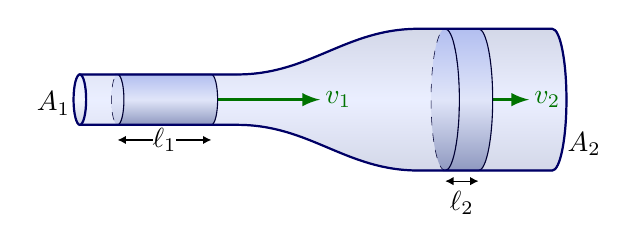
\begin{tikzpicture}
  \def\LL{2.0}         % length pipe left
  \def\LR{1.7}         % length pipe right
  \def\L{3.0*\LL}      % total length
  \def\l{\L-\LL-\LR}   % length between pipes
  \def\xL{0.24*\LL}    % position volume left
  \def\xR{\L-0.80*\LR} % position volume right
  \def\lL{0.7*\LR}     % length volume left
  \def\lR{\lL*\ry/\Ry} % length volume right
  \def\rx{0.08}        % small pipe horizontal radius left
  \def\ry{0.32}        % small pipe vertical radius left
  \def\Rx{0.18}        % big pipe vertical radius right
  \def\Ry{0.90}        % big pipe vertical radius right
  \def\v{1.3}          % velocity magnitude
  
  % WATER
  \draw[horizontal water]
    (0,\ry) -- (0,-\ry)  coordinate (A1) --++ (\LL,0) to[out=0,in=180]
    (\L-\LR,-\Ry) -- (\L,-\Ry) coordinate (A2) arc(-90:90:{\Rx} and \Ry)
    --++ (-\LR,0)  to[out=180,in=0] (\LL,\ry) -- cycle;
  \node[above left] at (A1) {$A_1$};
  \node[above right=2] at (A2) {$A_2$};
  
  % VOLUMES
  \draw[vvec] (\xL+\lL+\rx,0) --++ (\v,0) node[right=-2] {$v_1$};
  \draw[vvec] (\xR+\lR+\Rx,0) --++ (\v*\ry/\Ry,0) node[right=-2] {$v_2$};
  \draw[dark water,dashed,very thin]
    (\xL,0) ellipse({\rx} and \ry)
    (\xR,0) ellipse({\Rx} and \Ry);
  \draw[dark water]
    (\xL,\ry) arc(90:-90:{\rx} and \ry) --++ (\lL,0)
              arc(-90:90:{\rx} and \ry) -- cycle;
  \draw[dark water]
    (\xR,\Ry) arc(90:-90:{\Rx} and \Ry) --++ (\lR,0)
              arc(-90:90:{\Rx} and \Ry) -- cycle;
  \draw[width]
    (\xL,-1.6*\ry) --++ (\lL,0) node[midway,fill=white,inner sep=0] {$\ell_1$};
  \draw[width]
    (\xR,-1.15*\Ry) --++ (\lR,0) node[midway,below] {$\ell_2$};
  
  % CONTAINER
  \draw[mydarkblue,thick]
    (0,\ry) -- (0,-\ry)  coordinate (A1) --++ (\LL,0) to[out=0,in=180]
    (\L-\LR,-\Ry) -- (\L,-\Ry) coordinate (A2) arc(-90:90:{\Rx} and \Ry)
    --++ (-\LR,0)  to[out=180,in=0] (\LL,\ry) -- cycle;
  \draw[water,thick]
    (0,0) ellipse({\rx} and \ry);
  
\end{tikzpicture}


% BERNOUILLI EQUATION
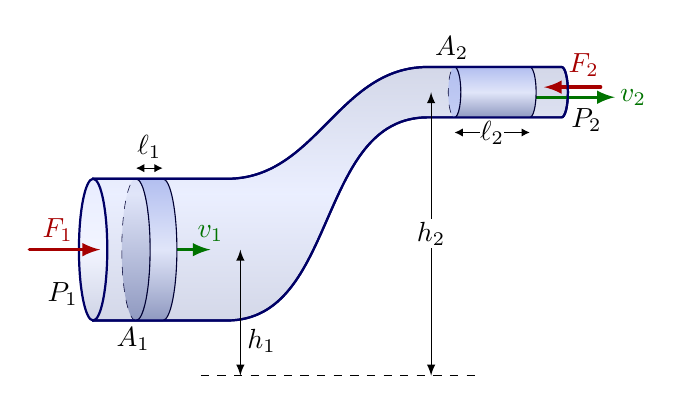
\begin{tikzpicture}
  \def\LL{1.7}          % length pipe left
  \def\LR{1.7}          % length pipe right
  \def\L{3.5*\LL}       % total length
  \def\H{2.0}           % height
  \def\l{\L-\LL-\LR}    % length between pipes
  \def\xL{0.32*\LL}     % position volume left
  \def\xR{\L-0.80*\LR}  % position volume right
  \def\lL{0.2*\LR}      % length volume left
  \def\lR{\lL*\Ry/\ry}  % length volume right
  \def\rx{0.08}         % small pipe horizontal radius left
  \def\ry{0.32}         % small pipe vertical radius left
  \def\Rx{0.18}         % big pipe vertical radius right
  \def\Ry{0.90}         % big pipe vertical radius right
  \def\v{1.0}           % velocity magnitude
  \def\F{0.9}           % force magnitude
  \def\y{(\Ry+0.35*\H)} % height from ground
  
  % WATER
  \draw[horizontal water,thick]
    (0,\Ry) -- (0,-\Ry) coordinate (P1) --++ (\LL,0) to[out=0,in=180]
    (\L-\LR,\H-\ry) -- (\L,\H-\ry) coordinate (P2) arc(-90:90:{\rx} and \ry)
    --++ (-\LR,0)  to[out=180,in=0] (\LL,\Ry) -- cycle;
  \node[above left=2] at (P1) {$P_1$};
  \node[above=-1,right=0] at (P2) {$P_2$};
  
  % VOLUMES
  \draw[vvec] (\xL+\lL+\Rx,0) --++ (\v*1.2*\ry/\Ry,0) node[above=-1] {$v_1$};
  \draw[vvec] (\xR+\lR+\rx,\H-0.2*\ry) --++ (\v,0) node[right=-2] {$v_2$};
  \draw[force] (\L-0.7*\ry+0.8*\F,\H+0.2*\ry) --++ (-0.8*\F,0) node[pos=0.3,above] {$F_2$};
  \draw[dark water,dashed,very thin]
    (\xL,0) ellipse({\Rx} and \Ry)
    (\xR,\H) ellipse({\rx} and \ry);
  \draw[dark water]
    (\xL,\Ry)
      arc(90:-90:{\Rx} and \Ry) coordinate (A1) --++ (\lL,0)
      arc(-90:90:{\Rx} and \Ry) -- cycle;
  \draw[dark water]
    (\xR,\H+\ry) coordinate (A2)
      arc(90:-90:{\rx} and \ry) --++ (\lR,0)
      arc(-90:90:{\rx} and \ry) -- cycle;
  \draw[width]
    (\xL,1.15*\Ry) --++ (\lL,0) node[midway,above] {$\ell_1$};
  \draw[width]
    (\xR,\H-1.6*\ry) --++ (\lR,0) node[midway,fill=white,inner sep=0] {$\ell_2$};
  \node[left=1,below=-1] at (A1) {$A_1$};
  \node[left=1,above=-1] at (A2) {$A_2$};
  
  % CONTAINER
  \draw[mydarkblue,thick]
    (0,\Ry) -- (0,-\Ry)  coordinate (A1) --++ (\LL,0) to[out=0,in=180]
    (\L-\LR,\H-\ry) -- (\L,\H-\ry) coordinate (A2) arc(-90:90:{\rx} and \ry)
    --++ (-\LR,0)  to[out=180,in=0] (\LL,\Ry) -- cycle;
  \draw[water,thick]
    (0,0) ellipse({\Rx} and \Ry);
  
  % HEIGHT
  \draw[dashed] (0.23*\L,{-\y}) --++ (0.6*\L,0);
  \draw[<->]
    (1.1*\LL,{-\y}) --++ (0,{\y}) node[pos=0.13,above right=-1] {$h_1$};
  \draw[<->]
    (0.95*\xR,{-\y}) --++ (0,{\H+\y}) node[midway,fill=white,inner sep=1] {$h_2$};
  \draw[force] (0.1*\Ry-\F,0) --++ (\F,0) node[pos=0.4,above=-1] {$F_1$};
  
\end{tikzpicture}



% VENTURI EFFECT
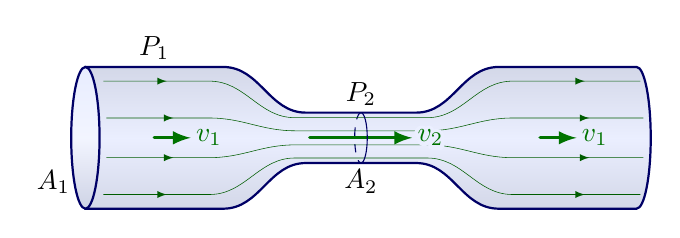
\begin{tikzpicture}
  \def\L{7.0}          % total length
  \def\m{0.20*\L}      % length pipe middle
  \def\l{0.25*\L}      % length pipe outer
  \def\rx{0.08}        % small pipe horizontal radius left
  \def\ry{0.32}        % small pipe vertical radius left
  \def\Rx{0.18}        % big pipe vertical radius right
  \def\Ry{0.90}        % big pipe vertical radius right
  \def\v{1.3}          % velocity magnitude
  \contourlength{1.5pt}
  
  % WATER
  \draw[horizontal water,thick]
    (-\L/2,\Ry) --++ (0,-2*\Ry) coordinate (A1) --++ (\l,0) to[out=0,in=180]
    (-\m/2,-\ry) --++ (\m,0) to[out=0,in=180]
    (\L/2-\l,-\Ry) --++ (\l,0) arc(-90:90:{\Rx} and \Ry) --++ (-\l,0) to[out=180,in=0]
    (\m/2,\ry) --++ (-\m,0) to[out=180,in=0] (-\L/2+\l,\Ry) -- cycle;
  \draw[water,thick]
    (-\L/2,0) ellipse({\Rx} and \Ry);
  \node[above left=2] at (A1) {$A_1$};
  \node[below=-1] at (0,-\ry) {$A_2$};
  
  % VELOCITIES
  \draw[mydarkblue,dashed]
    (0,\ry) arc(90:270:{\rx} and \ry);
  \foreach \fy in {-0.28,-0.8,0.28,0.8}{
    \coordinate (A) at ($(-\L/2,0)+({asin(\fy/1.5)}:{1.5*\Rx} and {1.5*\Ry})$);
    \coordinate (B) at ($({\L/2-\Rx},0)+({asin(\fy/1.5)}:{1.5*\Rx} and {1.5*\Ry})$);
    \draw[vcol!80!black,very thin,postaction={decorate},decoration={markings,
      mark=at position {0.13-0.02*abs(\fy)} with {\arrow{latex}},mark=at position 0.9 with {\arrow{latex}}}]
      (A) -- (-\L/2+0.9*\l,\fy*\Ry) to[out=0,in=180]
      (-0.6*\m,\fy*\ry) -- (0.6*\m,\fy*\ry) to[out=0,in=180] (\L/2-0.9*\l,\fy*\Ry) -- (B);
  }
  \draw[vvec] (-\L/2+0.5*\l,0) --++ (\v*\ry/\Ry,0) node[right=-2] {$v_1$};
  \draw[vvec] ( \L/2-0.7*\l,0) --++ (\v*\ry/\Ry,0) node[right=-2] {$v_1$};
  \draw[vvec] (-0.5*\v,0) --++ (\v,0) node[right=-2] {\contour{watercol!80}{$v_2$}};
  \draw[mydarkblue]
    (0,\ry) arc(90:-90:{\rx} and \ry);
  \node[above=-1] at (-\L/2+0.5*\l,\Ry) {$P_1$};
  \node[above=-1] at (0,\ry) {$P_2$};
  
  
\end{tikzpicture}


\end{document}
